\chapter{Experimente}
\label{cha:experimente}

\section{Vereinfachte Kalibrierung}
\label{sec:vereinfachtekalib}

Eine andere M"oglichkeit, als in \ref{sec:kalibrierung} erl"autert, eine Kamera zu kalibrieren, ist mit Hilfe eines rechteckigen Kalibrierobjektes. In unserem Fall handelt es sich, wie in \ref{fig:klammern} zu sehen ist, um die Verpackung von Heftklammern.
 
\begin{figure}[H]
	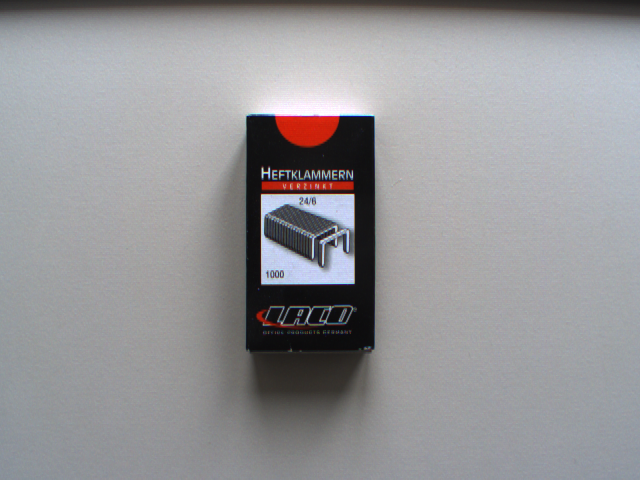
\includegraphics[scale=0.5]{bilder/experimentcalib}
	\caption[Kalibrierobjekt]{Kalibrierobjekt}
	\label{fig:klammern}
\end{figure}

\noindent Die Formel zur Berechnung der Brennweite $f_x$ und $f_y$ ergibt sich aus den Formeln

\begin{equation}
f_x=\frac{\Delta x'}{x}z
\end{equation}

und

\begin{equation}
f_y=\frac{\Delta y'}{y}z
\end{equation}

\noindent bei $\Delta x$ und $\Delta y$ handelt es sich um die jeweiligen Seitenl"angen des Kalibrierobjekts.\newline
$\Delta x'$ und $\Delta y'$ sind die L"angen der Seiten des Kalibrierobjekts in Pixelwerten. $z$ ist der Abstand zwischen Linse und Objekt \cite{PCV} \cite{CVF}.

\begin{figure}[H]
	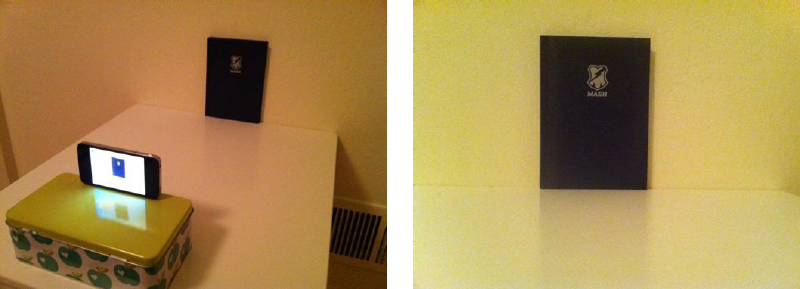
\includegraphics[scale=1.0]{bilder/simple_calib}
	\caption[Vereinfachte Kalibrierung]{Vereinfachte Kalibrierung}
	\small Quelle: Solem 2012
	\label{fig:simplecalib}%
\end{figure}

\noindent Wie in \ref{fig:simplecalib} zu sehen ist, muss das Kalibrierobjekt senkrecht auf eine plane Oberfl"ache gestellt werden. So auch die Kamera. Die Kamera muss dann so ausgerichtet werden, dass das Objekt im Bild genau zentriert und entlang der Bildzeilen und -spalten ausgerichtet ist \cite{CVF}.\newline
Obwohl diese Kalibrierung sehr ungenau erscheint, wurde ein dennoch relativ geringer Reprojection-Error errechnet. Der wie in \ref{sec:kalibrierung} ermittelte Wert war dennoch besser.

\section{Fehlerfortpflanzung}
\label{sec:fehlerfortpflanzungtiefen}

Bei der Tiefenberechnung mit Hilfe eines Stereokamerasystems wird die Raumposition nicht gemessen, sondern aus den beiden vom Kamerasystem erfassten Bildern berechnet. Dazu wird der gleiche Raumpunkt in beiden Bildern detektiert. Die räumliche Rekonstruktion ist im Stereonormalfall besonders einfach, da die beiden Kameras keine Rotation zueinander aufweisen. Dadurch vereinfachen sich die allgemeinen Formeln zur räumlichen Rekonstruktion \cite{frz}

\begin{equation}
x = x_{0} + (z - z_{0})\frac
{r_{11}(x'-x_{0}') + r_{12}(y'-y_{0}')-r_{13}f}
{r_{31}(x'-x_{0}') + r_{32}(y'-y_{0}')-r_{33}f}
\end{equation}

\begin{equation}
y = y_{0} + (z - z_{0})\frac
{r_{21}(x'-x_{0}') + r_{22}(y'-y_{0}')-r_{23}f}
{r_{31}(x'-x_{0}') + r_{32}(y'-y_{0}')-r_{33}f}
\end{equation}

\noindent zu\newline
\noindent Rechtes Bild:
\begin{equation}\label{eq:one}
x = -z \frac{x'_{1}}{f}
\end{equation}
\begin{equation}\label{eq:two}
y = -z \frac{y'_{1}}{f}
\end{equation}

\noindent Linkes Bild:
\begin{equation}\label{eq:three}
x = B-z \frac{x'_{2}}{f}
\end{equation}
\begin{equation}\label{eq:four}
y = -z \frac{y'_{2}}{f}
\end{equation}

\noindent Aus den vereinfachten Formeln \ref{eq:one}, \ref{eq:two}, \ref{eq:three} und \ref{eq:four}, ist es ersichtlich, dass ein Raumpunkt in beiden Bildern die gleiche $y$-Koordinate aufweist, sich jedoch normalerweise in der $x$-Koordinate unterscheidet. Diese Differenz wird als $x$-Parallaxe 
$\rho_{x} = x_{1} - x_{2}$ oder Disparität $D$ bezeichnet.\newline
\noindent Durch Gleichsetzen der Formeln \ref{eq:one} – \ref{eq:four} für linkes und rechtes Bild, erhält man folgende Formel zur Berechnung der Tiefeninformation:

\begin{equation}\label{eq:tiefe}
z = -\frac
{f*B}
{x'_{1}-x'_{2}}
=
-\frac
{f*B}
{\rho x'}
\end{equation}

\noindent Da die Brennweite f und der Abstand der beiden Kameras zueinander (Baseline $B$) konstant sind, ist die Entfernung allein von der $x$-Parallaxe abhängig. Dabei ist ein Punkt näher, je größer die Parallaxe ist. \newline
Die Formel \ref{eq:tiefe} wurde mit folgendem Experiment validiert:


\begin{figure}[!htb]
	\minipage{0.32\textwidth}
	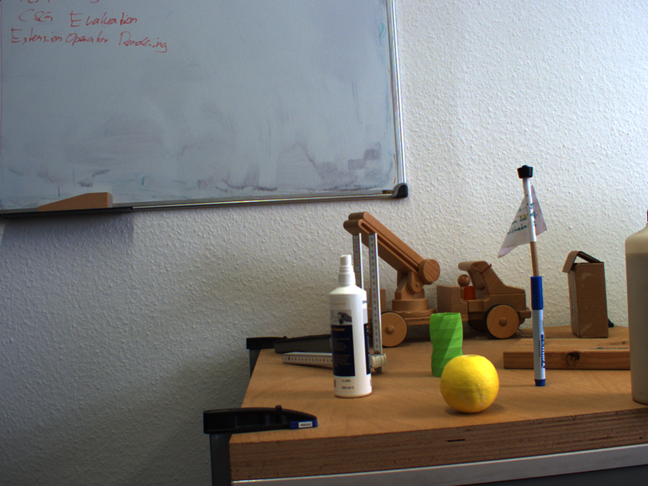
\includegraphics[width=\linewidth]{bilder/depth_left}
	\caption{Tiefe links}\label{fig:depthleft}
	\endminipage\hfill
	\minipage{0.32\textwidth}
	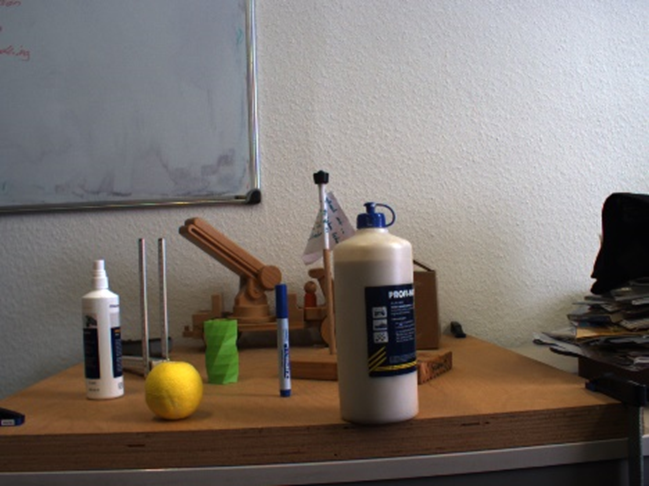
\includegraphics[width=\linewidth]{bilder/depth_right}
	\caption{Tiefe rechts}\label{fig:depthright}
	\endminipage\hfill
	\minipage{0.32\textwidth}%
	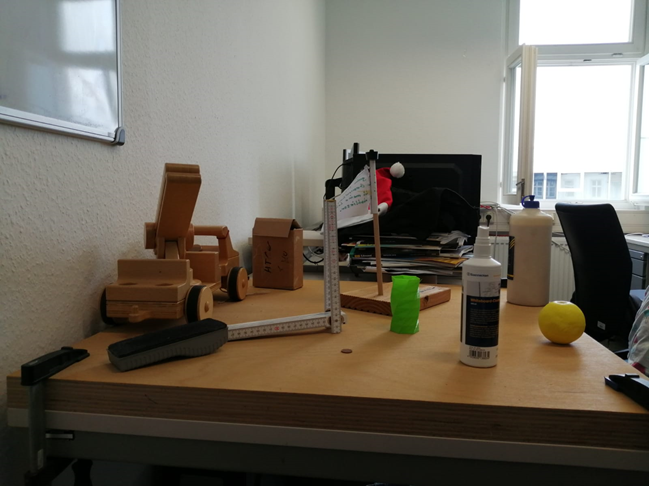
\includegraphics[width=\linewidth]{bilder/depth_side}
	\caption{Tiefe seitlich}\label{fig:depthside}
	\endminipage
\end{figure}

\noindent Mit dem Stereo-System wurden zwei Aufnahmen einer Szene aufgenommen (\ref{fig:depthleft} und \ref{fig:depthright}). Auf dem seitlichen Bild \ref{fig:depthside} sieht man die tats"achliche Tiefe der Objekte im Bild.

\begin{figure}[!htb]
	\minipage{0.48\textwidth}
	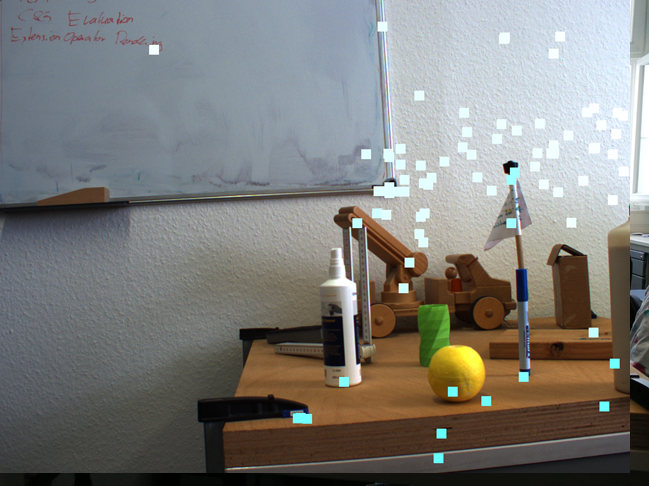
\includegraphics[width=\linewidth]{bilder/depth_result}
	\caption{Tiefeninformation Punkte}\label{fig:depthpoints}
	\endminipage\hfill
	\minipage{0.48\textwidth}
	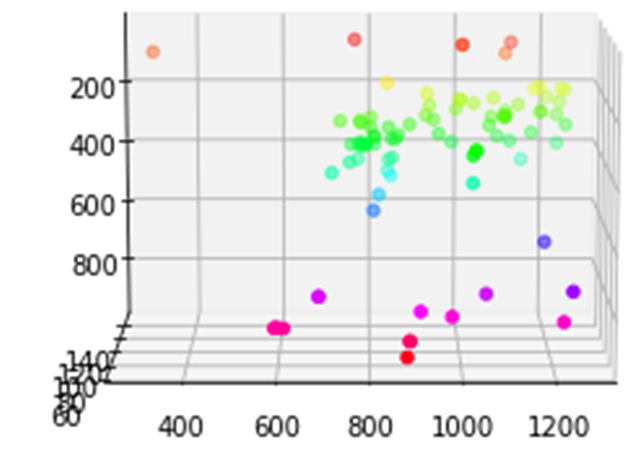
\includegraphics[width=\linewidth]{bilder/depth_coord}
	\caption{Tiefeninformation 3D-Plot}\label{fig:depthplot}
	\endminipage\hfill
\end{figure}

\noindent Auf den zwei Bildern der Szene wurden hier vorerst h"andisch, dann mittels des SIFT-Algorithmus Referenzpunkte ermittelt, zu denen die Tiefe berechnet werden sollte.\newline
\noindent Mittels eines selbst geschriebenem Algorithmus, der Werte mit im Mittel großem $z$ wei"slich und Werte mit im Mittel kleinem $z$ hellblau einf"arbt, kann man sich die Informationen zur Tiefe auf einem Bild darstellen. In \ref{fig:depthpoints} kann man gut erkennen, dass Objekte, die n"aher an der Kamera stehen, mit einem hellen blau markiert sind. Objekte, die weiter entfernt sind, mit einem wei"slichem Farbton.\newline
\noindent Dieses Verfahren der indirekten Bestimmung der Tiefeninformationen ist jedoch anfällig für Messfehler in den Bildposition. Die Fehlerfortpflanzung über die Werte $x$, $y$ und $z$ wird mit Hilfe des Gaußschen Fehlerfortpflanzungsgesetzes, welches den Einfluss mehrerer fehlerbehafteter Eingangsgrößen auf eine zu schätzende Ausgangsgröße beschreibt, berechnet.
Wird die Varianz der Ausgangsgröße $y$ über die fehlerbehafteten Eingangsgrößen $x_{1}$ bis $x_{n}$  abgeschätzt, lautet die allgemeine Form des Gaußschen Fehlerfortpflanzungsgesetzes:

\begin{equation}
F3
\end{equation}

\noindent Wendet man dieses Gesetz auf die Formeln \ref{eq:one} - \ref{eq:tiefe} an, erhält man folgende Fehlerabschätzung für die Größen $z$, $y$ und $z$ unter der Annahme, dass die Brennweite $f$ und die Baseline $B$ fehlerfrei sind \cite{frz}:

\begin{equation}
F4.3
\end{equation}

\section{Genauigkeitsabschätzung des Systems}
\label{sec:genauigkeit}

Zur Genauigkeitsbeurteilung haben wir drei Mal das gleiche Objekt in jeweils einem anderen Abstand zum Stereosystem aufgenommen. Dabei erhielten wir folgende Resultate: